\documentclass[12pt]{beamer}
\usepackage[T2A]{fontenc}
\usepackage[utf8]{inputenc}
\usepackage[english,russian]{babel}
\usepackage{amssymb,amsfonts,amsmath,mathtext, wasysym}
\usepackage{cite,enumerate,float,indentfirst}
\usepackage{makecell}
\usepackage{multirow}
\usepackage{graphicx}
\graphicspath{{../images/}{images/}{../Thesis/images/}} 
\usepackage{tikz}
\usepackage{calc}
\def\checkmark{\tikz\fill[scale=0.7](0,.35) -- (.25,0) -- (1,.7) -- (.25,.15) -- cycle;}
\def\checkmarksmall{\tikz\fill[scale=0.5](0,.35) -- (.25,0) -- (1,.7) -- (.25,.15) -- cycle;}
\newcommand{\cond}{\;|\;}
\newcolumntype{L}[1]{>{\raggedright\let\newline\\\arraybackslash\hspace{0pt}}m{#1}}
\newcolumntype{C}[1]{>{\centering\let\newline\\\arraybackslash\hspace{0pt}}m{#1}}
\newcolumntype{R}[1]{>{\raggedleft\let\newline\\\arraybackslash\hspace{0pt}}m{#1}}
%\usetheme[secheader]{Boadilla}
%\usecolortheme{seahorse}

\usetheme{Madrid}
\usecolortheme{whale}
\setbeamertemplate{enumerate items}[circle]
\setbeamertemplate{itemize items}[circle]

\makeatletter
\long\def\beamer@author[#1]#2{%
	\def\insertauthor{\def\inst{\beamer@insttitle}\def\and{\beamer@andtitle}%
		\begin{minipage}{\linewidth}#2\end{minipage}}%
	\def\beamer@shortauthor{#1}%
	\ifbeamer@autopdfinfo%
	\def\beamer@andstripped{}%
	\beamer@stripands#1 \and\relax
	{\let\inst=\@gobble\let\thanks=\@gobble\def\and{, }\hypersetup{pdfauthor={\beamer@andstripped}}}
	\fi%
}
\makeatother
\author[Кочуров М.В.]{%
	\begin{center}
		\large{Кочуров Максим}
	\end{center}
\vspace{1\baselineskip}
	\begin{flushright}
		Научный руководитель:\\
		доцент, к.э.н. Лукаш Е.Н.
	\end{flushright}%
}



\beamertemplatenavigationsymbolsempty

\newcommand{\todo}{\alert}
%%% Основные сведения %%%
\newcommand{\thesisAuthorLastName}{Кочуров}
\newcommand{\thesisAuthorOtherNames}{Максим Вадимович}
\newcommand{\thesisAuthorInitials}{М.В.}
\newcommand{\thesisAuthor}             % Диссертация, ФИО автора
{%
    \texorpdfstring{% \texorpdfstring takes two arguments and uses the first for (La)TeX and the second for pdf
        \thesisAuthorLastName~\thesisAuthorOtherNames% так будет отображаться на титульном листе или в тексте, где будет использоваться переменная
    }{%
        \thesisAuthorLastName, \thesisAuthorOtherNames% эта запись для свойств pdf-файла. В таком виде, если pdf будет обработан программами для сбора библиографических сведений, будет правильно представлена фамилия.
    }
}
\newcommand{\thesisAuthorShort}        % Диссертация, ФИО автора инициалами
{\thesisAuthorInitials~\thesisAuthorLastName}
%\newcommand{\thesisUdk}                % Диссертация, УДК
%{\todo{xxx.xxx}}
\newcommand{\thesisTitle}              % Диссертация, название
{Эконометрическое моделирование динамики корреляций доходностей финансовых стратегий}
\newcommand{\thesisSpecialtyNumber}    % Диссертация, специальность, номер
{38.03.01}
\newcommand{\thesisSpecialtyTitle}     % Диссертация, специальность, название
{Экономика}
\newcommand{\thesisDegree}             % Диссертация, ученая степень
{Бакалавр Экономики}
\newcommand{\thesisDegreeShort}        % Диссертация, ученая степень, краткая запись
{Бакалавр Экономики}
\newcommand{\thesisCity}               % Диссертация, город написания диссертации
{Москва}
\newcommand{\thesisYear}               % Диссертация, год написания диссертации
{2018}
\newcommand{\thesisOrganization}       % Диссертация, организация
{Московский государственный университет имени М.В.Ломоносова}
\newcommand{\thesisOrganizationShort}  % Диссертация, краткое название организации для доклада
{МГУ им. М.В.Ломоносова}

\newcommand{\thesisInOrganization}     % Диссертация, организация в предложном падеже: Работа выполнена в ...
{Московском государственном университете имени М.В.Ломоносова}

\newcommand{\supervisorFio}            % Научный руководитель, ФИО
{Лукаш Евгений Николаевич}
\newcommand{\supervisorRegalia}        % Научный руководитель, регалии
{доцент кандидат экономических наук}
\newcommand{\supervisorFioShort}       % Научный руководитель, ФИО
{Е.Н. Лукаш}
\newcommand{\supervisorRegaliaShort}   % Научный руководитель, регалии
{доцент к.э.н.}


\newcommand{\opponentOneFio}           % Оппонент 1, ФИО
{\todo{Фамилия Имя Отчество}}
\newcommand{\opponentOneRegalia}       % Оппонент 1, регалии
{\todo{доктор физико-математических наук, профессор}}
\newcommand{\opponentOneJobPlace}      % Оппонент 1, место работы
{\todo{Не очень длинное название для места работы}}
\newcommand{\opponentOneJobPost}       % Оппонент 1, должность
{\todo{старший научный сотрудник}}

\newcommand{\opponentTwoFio}           % Оппонент 2, ФИО
{\todo{Фамилия Имя Отчество}}
\newcommand{\opponentTwoRegalia}       % Оппонент 2, регалии
{\todo{кандидат физико-математических наук}}
\newcommand{\opponentTwoJobPlace}      % Оппонент 2, место работы
{\todo{Основное место работы c длинным длинным длинным длинным названием}}
\newcommand{\opponentTwoJobPost}       % Оппонент 2, должность
{\todo{старший научный сотрудник}}

\newcommand{\leadingOrganizationTitle} % Ведущая организация, дополнительные строки
{\todo{Федеральное государственное бюджетное образовательное учреждение высшего профессионального образования с~длинным длинным длинным длинным названием}}

\newcommand{\defenseDate}              % Защита, дата
{23 мая 2018~г.}
\newcommand{\defenseCouncilNumber}     % Защита, номер диссертационного совета
{\todo{Д\,123.456.78}}
\newcommand{\defenseCouncilTitle}      % Защита, учреждение диссертационного совета
{\todo{Название учреждения}}
\newcommand{\defenseCouncilAddress}    % Защита, адрес учреждение диссертационного совета
{\todo{Адрес}}
\newcommand{\defenseCouncilPhone}      % Телефон для справок
{\todo{+7~(0000)~00-00-00}}

\newcommand{\defenseSecretaryFio}      % Секретарь диссертационного совета, ФИО
{\todo{Фамилия Имя Отчество}}
\newcommand{\defenseSecretaryRegalia}  % Секретарь диссертационного совета, регалии
{\todo{д-р~физ.-мат. наук}}            % Для сокращений есть ГОСТы, например: ГОСТ Р 7.0.12-2011 + http://base.garant.ru/179724/#block_30000

\newcommand{\synopsisLibrary}          % Автореферат, название библиотеки
{\todo{Название библиотеки}}
\newcommand{\synopsisDate}             % Автореферат, дата рассылки
{\todo{DD mmmmmmmm YYYY года}}

% To avoid conflict with beamer class use \providecommand
\providecommand{\keywords}%            % Ключевые слова для метаданных PDF диссертации и автореферата
{}
      % Основные сведения


\title[Моделирование динамики]{\thesisTitle}
\institute[МГУ]{\small
	Экономический Факультет\\
	МГУ имени М.В.Ломоносова}
\date[23 мая 2018]{\small Москва, 23 мая 2018}

\begin{document}
\maketitle
\begin{frame}{Актуальность}
\begin{block}{Возрастающий интерес практиков}
	Новые хеджфонды агрегируют торговые стратегии для формирования из них портфелей:
	\begin{itemize}
		\item Фонд \href{https://www.quantopian.com}{Quantopian} (Boston, USA)
		\item Фонд \href{https://www.worldquant.com}{World Quant} (New York, USA)
	\end{itemize}
\end{block}
\begin{block}{Стандартная портфельная теория не применима}
	К стандартным предпосылки о стохастической волатильности, возможной динамики корреляций добавляются проблемы:
	\begin{itemize}
		\item Огромная база алгоритмов, сравнительно короткие ряды
		\item Алгоритмы создают люди: распределение доходностей до~и~после создания -- разные вещи
\end{itemize}
\end{block}
\textbf{Исследования, решающие эти проблемы, отсутствуют}
\end{frame}

\begin{frame}{Цель и Задачи}
\textbf{Цель:} разработка процедуры составления портфеля биржевых торговых стратегий, учитывающей априорные знания о распределении их доходностей

\textbf{Задачи:}

\begin{enumerate}
	\small
	\item Сформировать общую схему моделирования динамики торговых стратегий
	\item Предложить конкретные спецификации модели динамики доходностей
	\item Предложить метод оценки модели, реализовать его в виде программного продукта
	\item Предложить метод составления портфеля имея модель динамики
	\item На реальных данных выбрать адекватную спецификацию и оценить ее
	\item Сравнить разработанную процедуру с существующей, используемой на практике
\end{enumerate}
\end{frame}
\begin{frame}{Преимущества байесовского подхода}
\begin{minipage}{0.6\linewidth}
	\[\small p(\Theta\cond\mathcal{D}) =
	\frac
	{p(\mathcal{D}\cond\Theta)p(\Theta)}
	{p(\mathcal{D})}\]
	\begin{itemize}
		\item Учет экспертных знаний в априорном распределении $p(\Theta)$
		\item Интерпретируемость
		\item Гибкость моделирования
		\item Учет неуверенности при оценке параметров $p(\Theta\cond\mathcal{D})$
		\item Учет неуверенности при прогнозировании
	\end{itemize}
\end{minipage}
\begin{minipage}{0.38\linewidth}
	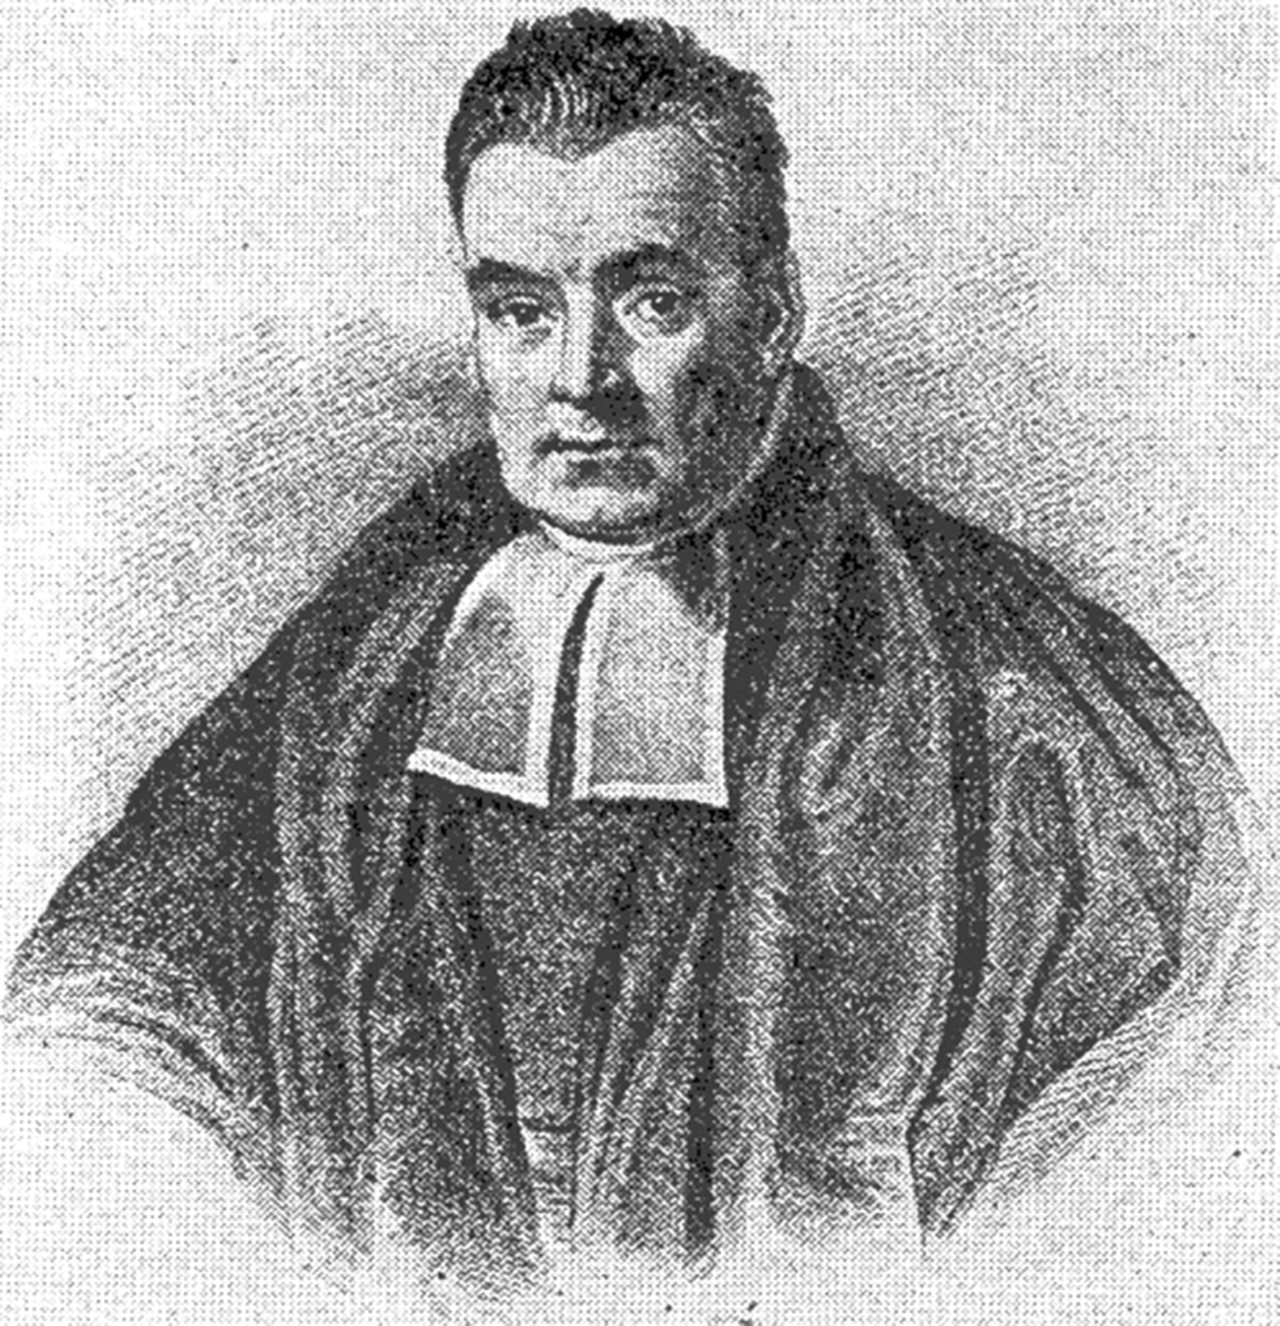
\includegraphics[width=\linewidth]{bayes}
\end{minipage}
\textbf{Основной недостаток:} сложность оценивания модели
\end{frame}
\begin{frame}{Выбор инструментов моделирования динамики доходностей}
\begin{block}{Динамика волатильности}
Модель  \textbf{GPVol} (волатильность $\sim$ гауссовский процесс)

\textbf{Преимущества:} богаче GARCH, интерпретируема и проста в использовани
\end{block}
\begin{block}{Динамика корреляций}
	\begin{tabular}{L{.5\linewidth}|L{.5\linewidth}}
		\textbf{DCC} & \textbf{DECO*} \checkmark\\
		($+$) полная динамика & ($-$) неполная динамика\\
		($-$) не масштабируется & ($+$) масштабируется\\
		& ($-$) требуется модификация
	\end{tabular}
\end{block}
* Предложена авторская модификация модели DECO c использованием гауссовского процесса
\end{frame}
\begin{frame}{Спецификация модели динамики доходностей}
\textbf{Ключевые компоненты:} \hfill Уравнения в раздатке:
\begin{itemize}
	\item Доходности $r_t$ $\sim$ Гауссовский Процесс (ГП) + Шум \hfill (12)
	\begin{itemize}
		\item[\checkmarksmall] среднее ГП -- \textbf{средняя доходность} \hfill (1--2)
	\end{itemize}
	\item Волатильность $\sigma_t$ $\sim$ Гауссовский Процесс \hfill (9)
	\begin{enumerate}
		\item[\checkmarksmall] Идеи GPVol
	\end{enumerate}
	\item Корреляции доходностей торговых стратегий
	\begin{enumerate}
		\item Динамические $\rightarrow$ модель DECO с ГП \hfill (14--15)
		\item Статические \hfill (17)
		\item Без корреляций \hfill (18)
	\end{enumerate}
	\item Структурный сдвиг (учет момента создания алгоритма)
	\begin{itemize}
		\item[\checkmarksmall] только для \textbf{средних доходностей} \hfill (1, 2, 12)
	\end{itemize}
\end{itemize}

\begin{block}{}
	При создании алгоритма преимущественное количество принимаемых во внимание показателей основывается именно на доходности
\end{block}
\end{frame}
\begin{frame}{Оценка байесовской модели}
Оценка байесовской модели -- вывод апостериорного распределения $p(\Theta\cond\mathcal{D})$
\[p(\Theta\cond\mathcal{D}) =
\frac
{p(\mathcal{D}\cond\Theta)p(\Theta)}
{p(\mathcal{D})}\]
Где:
\begin{itemize}
	\item $\mathcal{D}$ -- данные
	\item $p(\Theta)$ -- априорное распределение
	\item $p(\mathcal{D}|\Theta)$ -- правдоподобие
\end{itemize}
Получение выборки $\{\Theta_i\}\sim p(\Theta\cond\mathcal{D})$ -- Hamiltonian Monte Carlo
Симуляция будущих траекторий доходностей $d_{new}$:
\begin{align*}
\text{аналитически сложно}&\qquad p(d_{new}\cond\mathcal{D})=\int p(d_{new}|\Theta)p(\Theta\cond\mathcal{D}) d\Theta,\\
\text{или имея $\{\Theta_i\}$}&\qquad \{d_{new}^{ik}\} \sim p(d_{new}|\Theta_i)\qquad\text{легко}
\end{align*}
\end{frame}

\begin{frame}{Оптимизация портфеля}
Построение портфеля основывается на симуляции будущих траекторий доходностей методом \textbf{Монте--Карло}

\begin{minipage}{0.49\linewidth}
	\begin{enumerate}
		\item Оцениваем модель\\$\{\Theta_i\}\sim p(\Theta\cond\mathcal{D})$
		\item Делаем симуляции траекторий  доходностей алгоритмов\\$\{d_{new}^{ik}\} \sim p(d_{new}|\Theta_i)$ 
		\item Оптимизируем матожидание функции полезности инвестора по долям в портфеле $w$\\
		$\tfrac{1}{I\dot K}\sum_{i, k}U(d^{ik}_{new}, w)\to \underset{w}{max}$
	\end{enumerate}
\end{minipage}
\begin{minipage}{0.49\linewidth}
	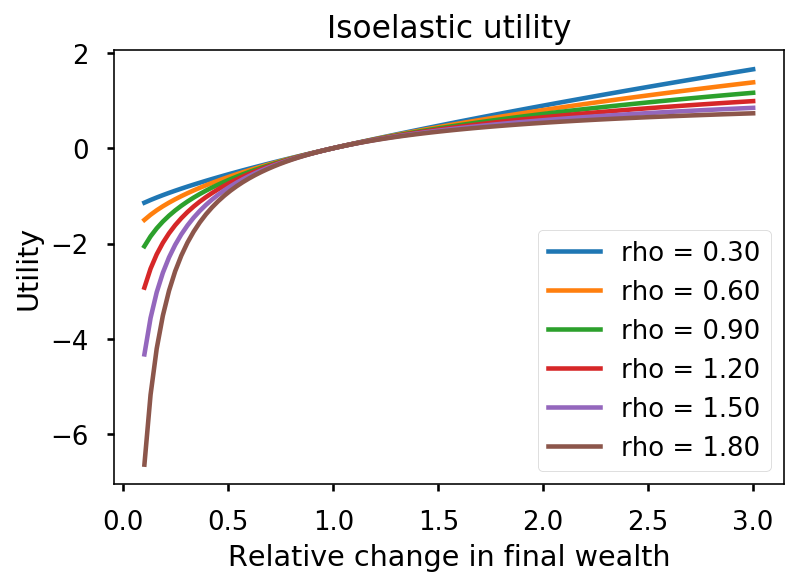
\includegraphics[width=\linewidth]{isoelastic}
	\centering
	
	Полезность инвестора
\end{minipage}
\end{frame}

\begin{frame}{Данные}
Данные были предоставлены компанией \textbf{Quantopian}
\begin{itemize}
	\item Всего более 700000 алгоритмов за период 4 года
	\item Существует внутренняя система отбора стабильных алгоритмов, отбирает около $0.05\%$
\end{itemize}
Эмпирические факты для отобранных алгоритмов:
\begin{itemize}
\item Наблюдается эффект не постоянной волатильности
	\item Корреляции довольно стабильны во времени
\end{itemize}
\textbf{Подходят только спецификации со статическими корреляциями}
\end{frame}
\begin{frame}{Описание процедуры сравнения эффективности}
Сравнивается эффективность предложенной процедуры с базовой (модель Марковица).

Критерий -- коэффициент Шарпа на отложенной выборке
\begin{itemize}
	\item Составление выборки
	\begin{itemize}
		\item Всего 4 года значений доходностей 150 финансовых стратегий от Quantopian
		\item Обучающая выборка -- первые два года
		\item Отложенная выборка -- последние два года
	\end{itemize}
	\item Подготовка бутстрап процедуры
	\begin{itemize}
		\item Сгенерировано 500+ выборок алгоритмов размера 20
	\end{itemize}
	\item Построение бутстрап распределения коэф. Шарпа
	\begin{itemize}
		\item Тремя методами: на основе моделей <<с корреляциями>>, <<без корреляций>> и по Марковицу, строятся портфели по данным обучающей выборки
		\item Считается критерий качества (коэффициент Шарпа) на отложенной выборке
	\end{itemize}
\end{itemize}
\end{frame}
\begin{frame}{Сравнительный анализ}
\textbf{Бутстрап распределение коэфф. Шарпа портфелей\\(отложенный период)}
\includegraphics[width=\linewidth]{performance-rus-1-1}
\end{frame}
\begin{frame}{Результаты исследования}
\begin{itemize}
	\item \textbf{Реализованы} спецификации модели \textbf{с учетом и без учета динамики корреляций}
	\item Для оценки модели динамики корреляций предложена \textbf{модификация базового метода DECO}
	\item Для определения адекватной спецификации модели \textbf{впервые} проведен эмпирический \textbf{анализ динамики корреляций доходностей торговых стратегий}
	\item \textbf{Предложен дизайн процедуры сравнения} для выявления практической значимости работы
	\item \textbf{Показана эффективность} использования байесовского подхода по сравнению с традиционно используемым
\end{itemize}
\end{frame}
\end{document}
